\section{Graph Partitioning for Distributed Memory}
\label{sec:partitions}


Outline:
\begin{itemize}
\item Rationale for why Hilbert ordering should be good for distributed memory
\item Show fraction of edges that cross partitions w/ and w/o Hilbert ordering
\end{itemize}

\begin{figure}[h]
\centering
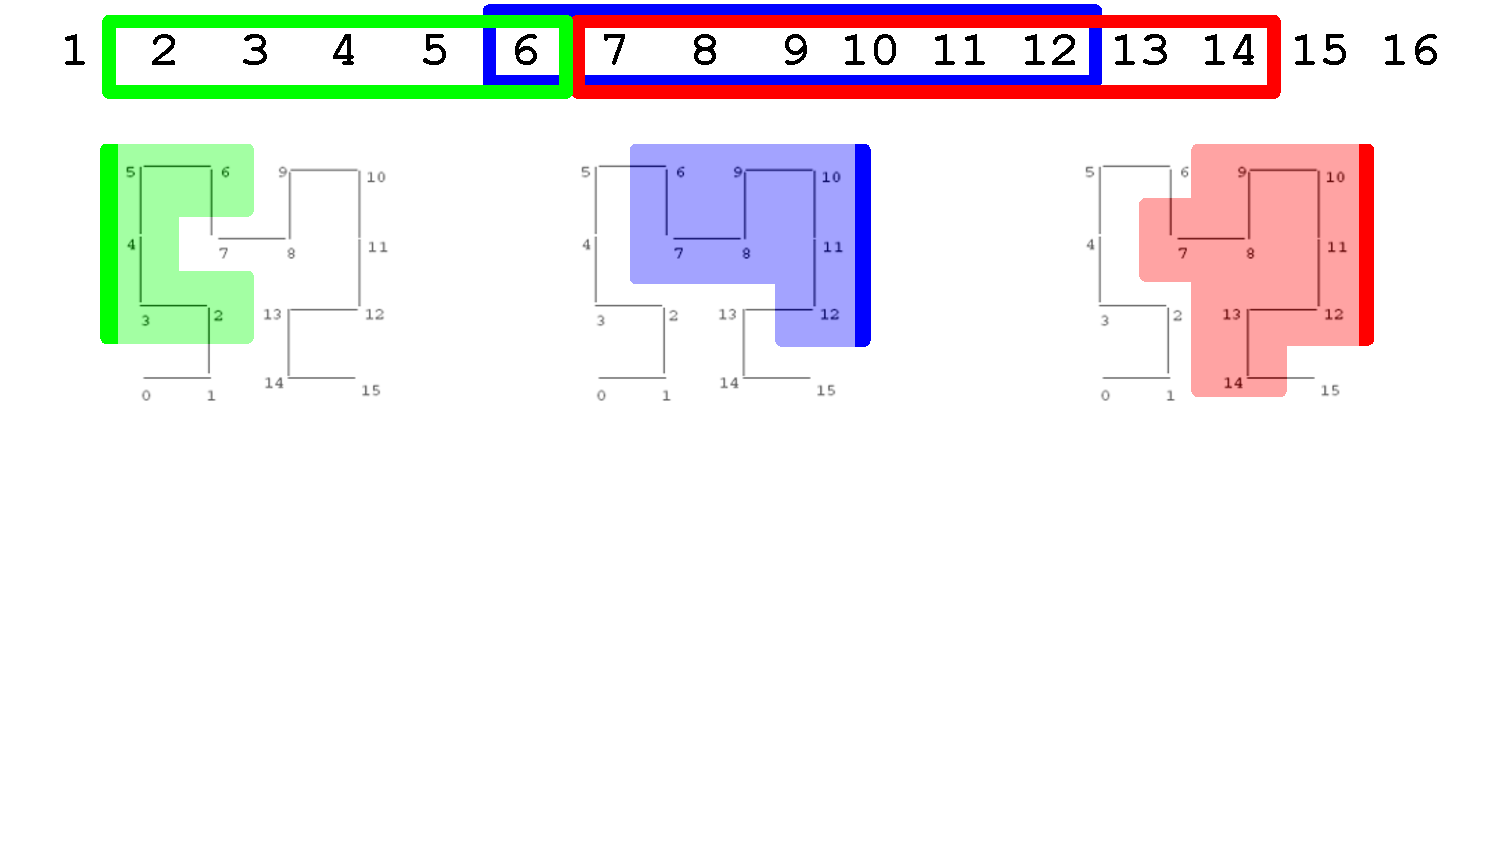
\includegraphics[width=5in,clip,trim=0 5cm 0 0]{hilbert_compact.pdf}
\caption{Examples of how contiguous subintervals yield compact
spaces in 2-dimensional space.}
\label{fig:hilbert_compact}
\end{figure}

\begin{figure}[h]
\centering
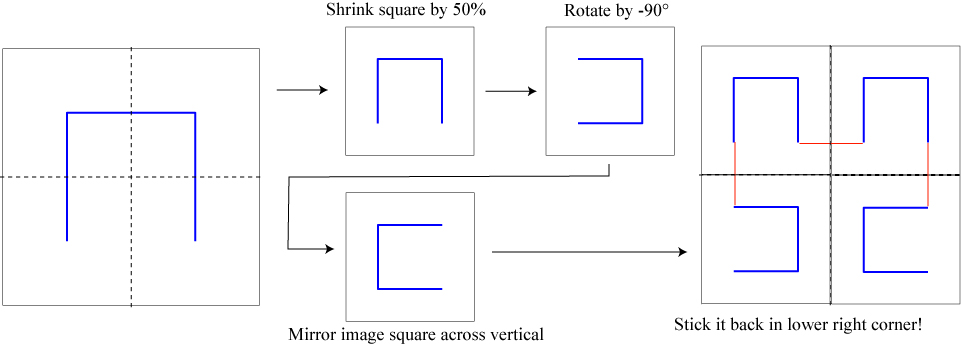
\includegraphics[width=5in,clip,trim=0 0 0 0]{fourthifs.jpg}
\caption{The construction of the Hilbert curve makes it
clear that contiguous subintervals of the curve yields
compact volumes in $N$-dimensional space: the curve always
makes 90 degree turns in an $N$-dimensional construction,
thus every pair of adjacent volumes in the Hilbert curve share a
face.}
\label{fig:hilbert_construction}
\end{figure}



In this section, we will describe how the Hilbert curve is also
a convenient mechanism for paritioning locally connected graphs
that are embeddable in a low-dimensional space.  That is, it 
generates a partition with small edge cuts.  We will discuss how
the priority-dag scheduling approach enables us to decompose the 
problem into two phases.  The first phase is to extend \proc{Prism}
to support a reshuffling operator, given a priority value from each
vertex, which re-organizes the graph data structure in linear order 
according to the priority function.  The second phase is to partition
the $n$ vertices by merely assigning $n/p$-sized compact subintervals
of vertices to each of the $p$ multi-core nodes.  Finally, we 
will describe the software architecture that integrates MPI commands
communicating over edges spanning partitions with the priority-dag 
scheduled computations on each multi-core node.  We will test the
performance of our implementation by measuring strong-scaling
performance on a small set of test graphs.


\section{Dealing with Distributed Execution}
Since an update function can only be run on a vertex if its 
neighbors are at most one iteration behind, we need to incur 
network traffic on every iteration to communicate vertex values 
for edges that cross machines. This can be done in a few ways. 
First, when an update function is being run on a vertex, it can 
fetch the values for neighbors on different machines and then 
run the necessary computation. This synchronous approach seems 
less than ideal, since the network traffic falls on the critical 
path of the iteration -- it is very likely that vertices that 
are capable of being updated without any network requests are 
waiting idle as the network requests complete.

Thus, an asynchronous approach is generally preferable. Our 
approach is as follows. For each edge that crosses machines, 
we declare one endpoint vertex as the predecessor and the other 
as the successor. Once the predecessor is updated, it sends 
its value to the machine to which the successor is assigned. 
Once the successor has received values from all of its 
predecessors, it can be scheduled for execution. If our 
partioning of vertices across machines is good and there are 
many vertices on each machine that have no dependencies on 
external vertices and therefore can be scheduled at any time, 
then there will be minimal waiting for network messages. Our 
scheme ensures that we satisfy the constraint that vertex 
updates must appear to be processed in some global order -- 
in other words, both of the endpoints of an edge cannot be 
updated in some iteration based on the other's data from 
the previous iteration.

\begin{figure}[!t]
\centering
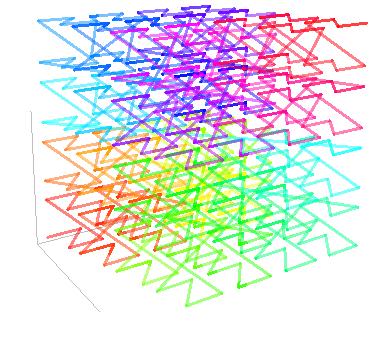
\includegraphics[width=2.5in]{z}
\caption{A Z-order curve tracing out the 3D space bounded by the box.}
\label{fig_z}
\end{figure}

We partition vertices across machines using a technique 
based on space-filling curves. A 3D space-filling curve 
maps the real numbers to points in 3D space so that for 
an arbitrary point $p$ as we trace out more and more of 
the curve the distance from $p$ to the nearest point on 
the curve becomes smaller and smaller. We use a Z-order 
curve, which has the property that if two points on the 
curve are relatively close together, then the real numbers 
that generated those points tend to be relatively close. A 
Z-order curve in 3D space is shown in Figure 2.

Each vertex in a mesh graph can be assigned a particular 
coordinate in 3D space. Thus, we can draw a bounding box 
in 3D space around a mesh graph. We trace out a Z-order 
curve over a finite portion of its domain mapping to points 
n the bounding box. We then assign each vertex in the mesh 
to its nearest point in the traced curve and mark the vertex 
with the real number that generated this point, which we will 
call the Z-number. We then sort the vertices by Z-number. 
Nearby vertices in the sorted order should be nearby in the 
physical graph. We can then split this sorted list into 
contiguous chunks, one for each machine in our cluster. 
Since each chunk should correspond to some contiguous 
region in 3D space, the number of edges crossing machines 
should be fairly small, as explained in the previous section.
